
Many important applications must process large streams of live data
and provide results in near-­real-­time.
Distributed  stream  processing  framework  is  required  to  scale  large
clusters  (100s  of  machines) and achieve  low  latency  (few  seconds).


\begin{tabular}{m{10cm}m{6cm}}
    Streaming  systems  have  a  record-at-a-time processing  model
    \begin{itemize}
        \item Each node has mutable state
        \item For  each  record,  update  state   and  
            send  new  records
    \end{itemize}
    &
    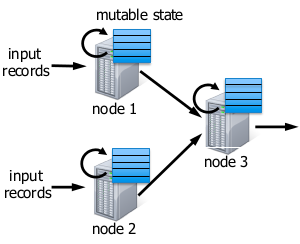
\includegraphics[width=5cm]{img/stream}
\end{tabular}

Note that state  is  lost  if  node  dies, so make a stateful stream
processing  be  fault-­tolerant  is  challenging.

\subsection{Storm}

Framework  for  distributed  stream  processing which provides:  
(1) stream  Partitioning, (2) fault  tolerance  and (3)  parallel  execution.
\begin{center}
    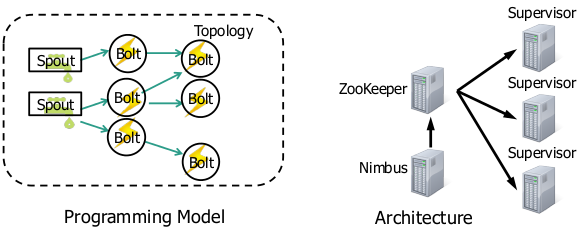
\includegraphics[width=10cm]{img/storm}
\end{center}

\begin{itemize}
    \item \textbf{Spout} is the source of stream where \textbf{bolt} process the stream
        and output new streams
    \item Nimbus  node  (master  node): 
        \begin{enumerate}
            \item Distributes  code,  launches  workers  across  the  cluster
            \item Monitors  computation  and  reallocates  workers  as  needed
        \end{enumerate}
    \item ZooKeeper nodes (coordinate  the  cluster)
    \item Supervisor  nodes: Start  and  stop  workers  according  to  signals
        from  Nimbus
\end{itemize}

\subsubsection{Fault tolerance}
Storm  can  guarantee  that  every  tuple  will  be  process  at  least  once or
at  most  once,  but  not  exactly  once. (Exactly  once  guarantee  requires
a  durable  data  source  that  can  replay  any  message  or  set  of
messages  given  the  necessary  selection  criteria)
%Suppose you want to update a counter in a database, if a worker fails, you 
% don't know if it has failed before updating the value or after 
%TODO really see slide 29 for 07 why this


If  a  supervisor  node  fails,  Nimbus  reassigns  that  node’s  task  to
other  nodes  in  the  cluster. Any  tuples  sent  to  a  failed  node  will
time  out  and  be  replayed. (Delivery  guarantee  dependent  on  a  reliable
data  source)

\subsection{Spark streaming}
Run  a  streaming  computation  as  a  series  of  
very  small,  deterministic  batch  jobs. This 
combine  the  efficiency  of  in-­memory  
distributed   processing  of  Spark  with  stream  
processing  mode.


\subsubsection{Work}

\begin{tabular}{m{10cm}m{6cm}}
    \begin{itemize}
        \item Chop  up  the  live  stream  into  batches  of  X  seconds  
        \item Spark  treats  each  batch  of  data  as  RDDs  and  processes  them
            using  RDD  operations
        \item Finally,  the  processed  results  of  the  RDD  operations  are
            returned  in  batches
    \end{itemize}
    &
    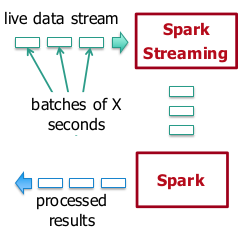
\includegraphics[width=4cm]{img/sparkStream}
\end{tabular}

At the end, a new RDDs are created for every batch

\subsubsection{Fault tolerance}

\begin{tabular}{m{10cm}m{6cm}}
    \begin{itemize}
        \item RDDs  remember  the  operations  that  created  them.
        \item Batches  of  input  data  are  replicated  in  memory  for
            fault-­tolerance.
        \item Data  lost  due  to  worker  failure,  can  be  recomputed  from
            replicated  input  data.
    \end{itemize}
    &
    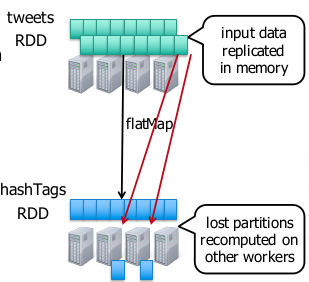
\includegraphics[width=6cm]{img/faultSpark}
\end{tabular}


